\section{Theory}
%\label{sec:problem_description}
There are three different types of flow meters, 
each with a pressure tube in front of and behind the 
meter to visualise the water pressure, as shown in figure \ref{Bf1},\ref{Bf2} and \ref{Bf3}.

The water enters from the venturi flow meter and flows through variable area, the orifice, 
then out of pipe. It should be noticed that there is an elbow between the venturi and variable area.

\begin{figure}
    \centering
\begin{minipage}[h]{0.33\textwidth} % Here, top, bottom priority list
    \centering
    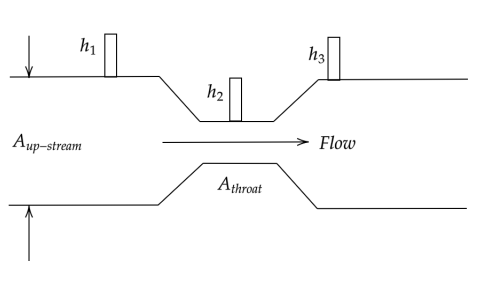
\includegraphics[scale=0.5]{Results/B1.png}
    \caption{Venture meter}
    \label{Bf1}
\end{minipage}
\begin{minipage}[h]{0.3\textwidth}% Here, top, bottom priority list
    \centering
    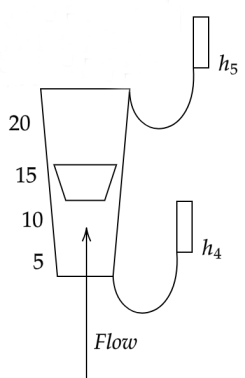
\includegraphics[scale=0.5]{Results/B3.png}
    \caption{Variable area meter}
    \label{Bf2}
\end{minipage}
\begin{minipage}[h]{0.33\textwidth} % Here, top, bottom priority list
    \centering
    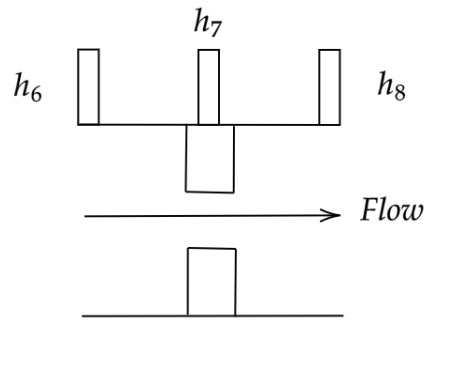
\includegraphics[scale=0.5]{Results/B2.png}
    \caption{Orifice plate meter}
    \label{Bf3}
\end{minipage}
\end{figure}

The definitions of the symbols are shown in table \ref{Bt1}.

\begin{minipage}[t]{\textwidth}
    \centering
\makeatletter\def\@captype{table}
\scalebox{1}{
\begin{tabular}{ccc}
    \toprule
    Symbols                     & Definition                   & Expression \\
    \midrule
    $H_{Qv} $                     & Head difference in venture                & $h_1-h_2 $     \\
    $H_{Qo} $                     & Head difference in orifice                 & $h_6-h_7 $    \\
    $H_v $                  & Head loss in venture                  & $h_1-h_3 $     \\
    $H_o $                   & Head loss in orifice                & $h_6-h_8 $   \\
    $H_a $                   & Head loss in variable area                & $h_4-h_5 $   \\
    $H_e $                   & Head loss in elbow               & $h_3-h_4 $   \\
   \bottomrule
\end{tabular}}
\caption{Symbol definitions}
\label{Bt1}
\end{minipage}




In Bernoulli's and continuity equations, for the venture meter,
\begin{equation}
    z_1+\frac{P_1}{\gamma}+\frac{v_1^2}{2g}=z_2+\frac{P_2}{\gamma}+\frac{v_2^2}{2g}
    \label{Be1}
\end{equation}
\begin{equation}
    Q_1=Q_2=A_1v_1=A_2v_2
    \label{Be2}
\end{equation}
Define $\Delta H$ as $h_1 - h_2 $, Hence,
\begin{equation}
    \Delta H=\left[z_1+\frac{P_1}{\gamma}\right]-\left[z_2+\frac{P_2}{\gamma}\right]
    \label{Be3}
\end{equation}
From equation \eqref{Bf1},\eqref{Bf2} and \eqref{Bf3}, 
\begin{equation}
    v_2=\sqrt{2g\Delta H}*\frac{A_1}{\sqrt{A_1^2-A_2^2}}
    \label{Be4}
\end{equation}
Due to the existence of discharge coefficients for the venturi and orifice, 
it is assumed that $C_d=0.98$ for venture and $C_d=0.63$ for orifice.
\begin{equation}
    Q_{actual}=C_d Q_{theoretical}=C_dA_2V_2=C_d\frac{A_1A_2}{\sqrt{A_1^2-A_2^2}}\sqrt{2g\Delta H}
    \label{Be5}
\end{equation}
Finally, the $Q_o$ and $Q_v$ could be write as
\begin{equation}
   Q_o=\frac{0.63A_2\sqrt{2g\Delta H_{Qo}}}{\sqrt{1-(\frac{A_2}{A_1})^2}}
    \label{Be6}
\end{equation}
\begin{equation}
    Q_v=\frac{0.98A_2\sqrt{2g\Delta H_{Qv}}}{\sqrt{1-(\frac{A_2}{A_1})^2}}
     \label{Be7}
 \end{equation}
 
For the variable area, there is a visual scale display.
This gives a very visibly readable indication of the flow of water.

For the elbow, head loss can be represented as 
\begin{equation}
    H_e=h_3-h_4=k\frac{v^2}{2g}
    \label{Be8}
\end{equation}
Which k is the coefficient of the elbow loss.


